\documentclass[../main.tex]{subfiles}

\begin{document}

\chapter{Deep Dive into Deep Neural Networks}

Neural networks (or neural nets) can be comprehended as a complex
function that does not require manual feature engineering.
Due to the high level of abstraction and automation in learning,
neural nets are highly scalable. This note covers neural nets with
mathematical interpretations and its application with Python.

\section{Definitions and High Level Overview}

As always, let's get started with the fundamental terms and high
level overview of what neural nets are. Before the introduction
of neural nets, traditional models like linear/logistic regression
and decision trees were used. The problem with traditional models
is that you are likely required to manually adjust the
\textbf{features}. With neural nets, the features are automatically
engineered, making us to focus on the architecture.

\subsection{High Level Architecture}
To understand the high level architecture, consider the diagram below.

\begin{figure}[H]
\centering
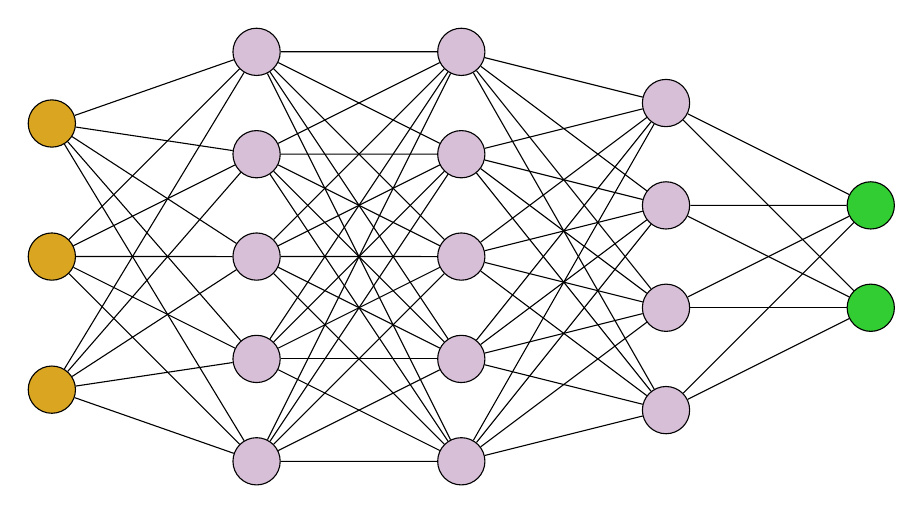
\begin{tikzpicture}[
    every node/.style={circle, draw, minimum size=0.6cm},
    input/.style={fill=Goldenrod},
    hidden/.style={fill=Thistle},
    output/.style={fill=LimeGreen},
    scale=1.3
]

    % Input Layer
    \node[input] (i1) at (0, 2.3) {};
    \node[input] (i2) at (0, 1) {};
    \node[input] (i3) at (0, -0.3) {};

    % Hidden Layer 1
    \node[hidden] (h1) at (2, 3) {};
    \node[hidden] (h2) at (2, 2) {};
    \node[hidden] (h3) at (2, 1) {};
    \node[hidden] (h4) at (2, 0) {};
    \node[hidden] (h5) at (2, -1) {};

    % Hidden Layer 2
    \node[hidden] (h6) at (4, 3) {};
    \node[hidden] (h7) at (4, 2) {};
    \node[hidden] (h8) at (4, 1) {};
    \node[hidden] (h9) at (4, 0) {};
    \node[hidden] (h10) at (4, -1) {};

    % Hidden Layer 3
    \node[hidden] (h11) at (6, 2.5) {};
    \node[hidden] (h12) at (6, 1.5) {};
    \node[hidden] (h13) at (6, 0.5) {};
    \node[hidden] (h14) at (6, -0.5) {};

    % Output Layer
    \node[output] (o1) at (8, 1.5) {};
    \node[output] (o2) at (8, 0.5) {};

    % Connections 
    \foreach \i in {1, 2, 3} {
        \foreach \j in {1, 2, 3, 4, 5} {
            \draw (i\i) -- (h\j);
        }
    }
    \foreach \i in {1, 2, 3, 4, 5} {
        \foreach \j in {6, 7, 8, 9, 10} {
            \draw (h\i) -- (h\j);
        }
    }
    \foreach \i in {6, 7, 8, 9, 10} {
        \foreach \j in {11, 12, 13, 14} {
            \draw (h\i) -- (h\j);
        }
    }
    \foreach \i in {11, 12, 13, 14} {
        \foreach \j in {1, 2} {
            \draw (h\i) -- (o\j);
        }
    }
\end{tikzpicture}
\caption{A visualization of a vanilla neural network (MLP)}
\end{figure}

From now, let's refer to the nodes as \textbf{neurons}.

\begin{definition}{}{}
\textbf{Neurons} are the fundamental unit in neural networks
that process input into output with set of parameters.
\end{definition}

From the diagram, the neurons are organized in to different
columns. We call the columns \textbf{layers}.

\begin{definition}{}{}
The \textbf{input layer} is the layer that receives inputs
for the neural network. \textbf{Hidden layers} are where the
input data is processed with the learned parameters to extract
information. The \textbf{output layer} is the final layer that
represents the final prediction of the neural network.
\end{definition}

In the diagram above, the input layer is represented as the
layer with yellow neurons, hidden layers as the layers with
purple neurons, output layer with the layer with green neurons.
One of the advantages of neural network is that there is simply
no limit, except computational limit. You can have unlimited
amount of neurons in each layers and unlimited amount of hidden
layers. The best neural net will be effectively structured in
a way that there are sufficient neurons to learn from while
avoiding overfitting and decreasing computational cost.

\begin{definition}{}{}
\textbf{Connections} are the links that connects the neurons
with each other.
\end{definition}

Just as our biological neurons are interconnected to each other,
artificial neurons are connected to effectively extract the
holistic feature from the input. Now it is worth noting that
each neuron represents \textbf{feature}.

Here is a brief example. Say your neural net will classify
handwritten numbers. The number $9$ and $0$ retains a similar
feature. Both the numbers have a loop in the top. Therefore,
in this scenario, the initial hidden layers may have similar
features when categorizing the numbers.

In the past we used \textbf{perceptrons}, or neurons that uses
step functions with binary output. However, modern multilayer
perceptron (MLP) uses a more flexible neurons with continuous
activation functions. Now let's take a look at what individual
neurons have with the diagram below.

\begin{figure}[H]
\centering
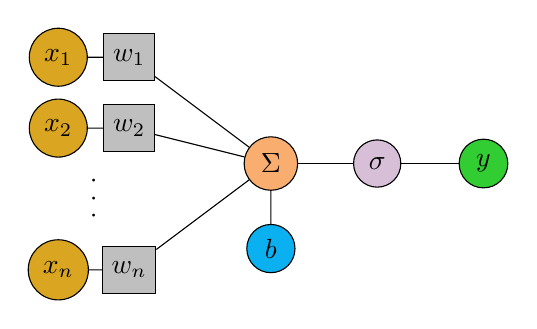
\begin{tikzpicture}[
    every node/.style={draw, minimum size=0.6cm},
    input/.style={circle, fill=Goldenrod},
    weight/.style={rectangle, fill=lightgray},
    bias/.style={circle, fill=ProcessBlue},
    sum/.style={circle, fill=Apricot},
    activation/.style={circle, fill=Thistle},
    output/.style={circle, fill=LimeGreen},
    scale=0.9
]

    \node[input] (x1) at (0, 2) {$x_1$};
    \node[input] (x2) at (0, 1) {$x_2$};
    \node[input] (xn) at (0, -1) {$x_n$};

    \node[draw=none] at (0.5, 0.25) {$\cdot$};
    \node[draw=none] at (0.5, 0) {$\cdot$};
    \node[draw=none] at (0.5, -0.25) {$\cdot$};

    \node[weight] (w1) at (1, 2) {$w_1$};
    \node[weight] (w2) at (1, 1) {$w_2$};
    \node[weight] (wn) at (1, -1) {$w_n$};
    \node[bias] (b) at (3, -0.7) {$b$};

    \node[sum] (sum) at (3, 0.5) {$\Sigma$};
    \node[activation] (act) at (4.5, 0.5) {$\sigma$};
    \node[output] (out) at (6, 0.5) {$y$};

    \draw (x1) -- (w1) -- (sum);
    \draw (x2) -- (w2) -- (sum);
    \draw (xn) -- (wn) -- (sum);
    \draw (b) -- (sum);
    \draw (sum) -- (act);
    \draw (act) -- (out);
\end{tikzpicture}
\caption{Visualization of a single neuron}
\end{figure}

On the high level, an individual neuron takes the weighted
sum of the previous layer with the trained parameter.
Bias is then added to make the activations more flexible.
Then, an activation function is used to determine the final
activation of the neuron.

\begin{definition}{}{}
\textbf{Activation} of a neuron indicates the significance of
a neuron, or presence of a feature from the input data.
An \textbf{activation function} is a function that generalizes
each activation and introduce \textbf{non-linearity}.
\end{definition}

In the diagram above, the purple color represents the activation
function and the green color represents the final output of
the neuron. Here, non-linearity is important for generalization
with activation function. The activation is represented as
a linear weighted sum. However, for generalization, activation
functions like ReLU (Sigmoid is considered outdated) are used.

Here, the superscript represents the layer and $i$ identifies the
neuron in the layer. The function $\sigma$ is an activation function.
It could be sigmoid, ReLU, tanh, and other activation functions.

\subsection{Training}

Inference is rather straight forward, but how do we ``train''
a model? Well, that's what this part of the note is all about.
There are few terminologies that we need to know, and I think
we can discuss them as we go along.

\begin{definition}{}{}
\textbf{Forward pass}, also known as \textbf{forward propagation},
the process of generating output with input data.
\end{definition}

Here, it is worth noting that forward pass is different from
inference in a sense that the process of inference only applies
to a complete trained model while forward pass also applies to
models being trained.

Let's discuss the definitions and underlying concepts in individual
process after capturing the big picture. Generally speaking,
the following diagram captures the training process.

\begin{figure}[H]
\centering
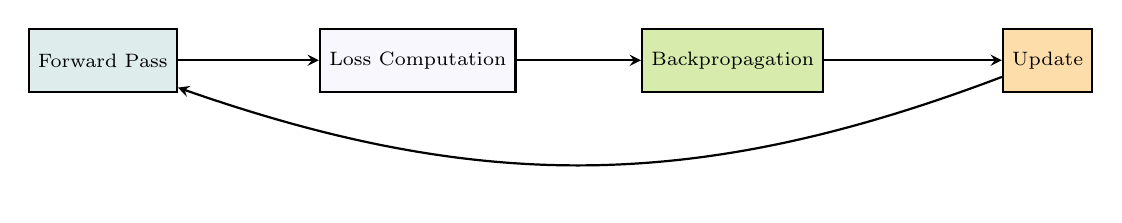
\begin{tikzpicture}[
    box/.style={rectangle, draw, thick,
                minimum height=0.8cm},
    arrow/.style={->, thick, >=stealth}
]

    \node[box, fill=CadetBlue!20] at (0, 0) (forward)
        {\scriptsize Forward Pass};
    \node[box, fill=Lavender!30] at (4, 0) (loss)
        {\scriptsize Loss Computation};
    \node[box, fill=YellowGreen!40] at (8, 0) (backprop)
        {\scriptsize Backpropagation};
    \node[box, fill=YellowOrange!30] at (12, 0) (update)
        {\scriptsize Update};

    \draw[arrow] (forward) -- (loss);
    \draw[arrow] (loss) -- (backprop);
    \draw[arrow] (backprop) -- (update);
    \draw[arrow, bend left=20] (update) to (forward);
\end{tikzpicture}
\caption{Overview of the Training Process}
\end{figure}

The first thing that we do after the forward pass is to calculate
the \textbf{loss}.

\begin{definition}{}{}
\textbf{Loss functions} are algorithms that calculate the
\textbf{loss}, or the performance of the prediction compared to
the expected outcome.
\end{definition}

There are many loss functions, but the two dominant functions are
\textbf{mean squared error (MSE)} and \textbf{cross-entropy} (a.k.a.
negative log-likelihood.) Generally, MSE is great for regression
and cross-entropy excels at classification. Therefore, cross-entropy
will commonly be used for LLMs for token predictions. Let's take a
look at each functions.

Following the convention, let $\hat{y}_n$ and $y_n$ be the prediction
and the true value respectively. With MSE, the loss will be
represented as $\frac{1}{n} \sum (\hat{y}_i - y_i)^2$. The intuition
behind this formula is we always want the loss to be positive as
it is comfortable to think that our goal is to reduce the loss.
If the loss is negative, it will be hard to apply this sense.
That's why we squared the difference. Now you might ask, why not
absolute value? Indeed, there is a function Mean Absolute Error (MAE),
but we like to square the values as it amplifies the loss.
With cross-entropy, its a bit more complicated, but a simplified
version would be $\sum (-y_i \log(\hat{y_i}))$. More on cross-entropy
will be discussed soon!

We know we can calculate the loss, but how do we actually improve
the model with the calculated loss?

\begin{definition}{}{}
An \textbf{optimizer} is an algorithm that determines the necessary
changes for model weights.
\end{definition}

The dominant optimizer type is \textbf{gradient descent} with its
variants like Adam, RMSProp, and SGD. There's quite a bit of content
for gradient descent for ML, so let's discuss that in a separate
section of the note.

\subsection{Gradient Descent and Learning Rate}

Before we implement the ideas and concepts above with code, I wanted
to discuss gradient descent and training more in-depth to actually
train our model. The partial derivatives and mathematical definition
of gradient descent was discussed in the first note. Here, we will
discuss about gradient descent specifically for ML.

\begin{definition}{}{}
\textbf{Gradient descent} as an optimizer represents how the weights
and biases of a model are updated based on the gradients of the loss
function.
\end{definition}

You would typically start from a random position to move in the
opposite direction of the gradient of the loss function.
Before I introduce mathematical equation, here are two famous
analogies of a ball rolling down the hill and finding a way in a
foggy forest. Starting with the first analogy, consider the
diagram below.

\begin{figure}[H]
\centering
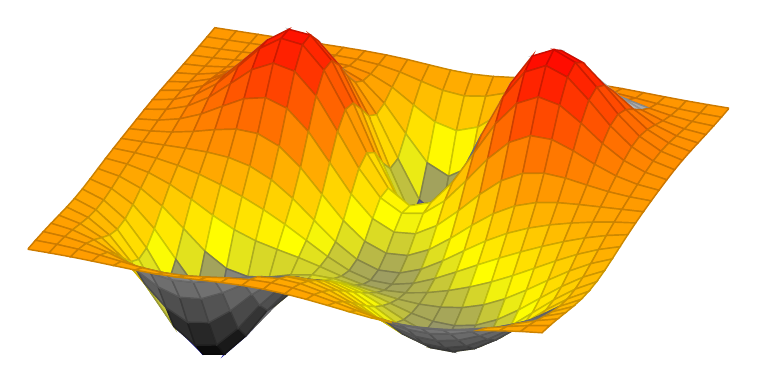
\begin{tikzpicture}[scale=1.3]
\begin{axis}[
        view={20}{40},
        hide axis,
        mesh/interior colormap name=hot,
        colormap/blackwhite,
    ]
    \addplot3 [domain=-2.5:2.5,surf] {
        -exp(-x^2 - y^2 - 0.05)
        -exp(-(x-1.2)^2 - (y+1.2)^2)
        -exp(-2*(x+1.2)^2 - 2*(y+1.2)^2 + 0.4) +
        -exp(-3*x^2 - 3*(y-1.5)^2 + 0.3) +
        exp(-2*(x+1.1)^2 - 2*(y-0.9)^2 + 0.06) +
        exp(-2*(x-1.2)^2 - 2*(y-1.2)^2 + 0.08)
    };
\end{axis}
\end{tikzpicture}
\caption{Ball Rolling Downhill Analogy}
\end{figure}

Imagine rolling a ball from the graph above. After some time, it will
naturally fall into one of the pits. If we are lucky, we will find
the global minimum, if not, we will fall into one of the local minima.
To see how we roll a ball, consider two diagrams below.

\begin{minipage}{0.48\textwidth}
\begin{figure}[H]
\centering
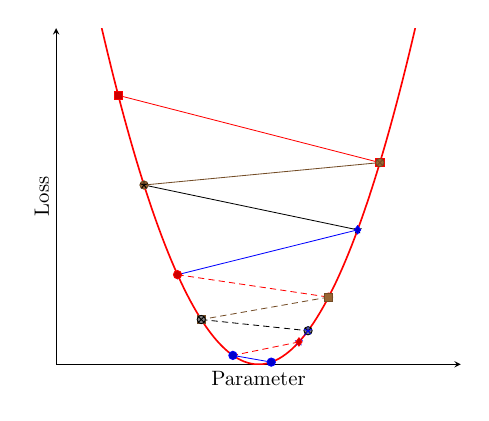
\begin{tikzpicture}[scale=0.75]
\begin{axis}[
        axis lines = left,
        xmin = 0,
        xmax = 10,
        xlabel = Parameter,
        ylabel = Loss,
        ticks = none
    ]
    \addplot [
        domain=1.12702:8.87298,
        samples=100,
        color=Red,
        thick
    ] {x^2 - 10*x + 25};
    \addplot coordinates {(1.5359,12) (8,9)};
    \addplot coordinates {(8,9) (2.17157,8)};
    \addplot coordinates {(2.17157,8) (7.44949,6)};
    \addplot coordinates {(7.44949,6) (3,4)};
    \addplot coordinates {(3,4) (6.73205,3)};
    \addplot coordinates {(6.73205,3) (3.58579,2)};
    \addplot coordinates {(3.58579,2) (6.22474,1.5)};
    \addplot coordinates {(6.22474,1.5) (6,1)};
    \addplot coordinates {(6,1) (4.36754,0.4)};
    \addplot coordinates {(4.36754,0.4) (5.31623,0.1)};
\end{axis}
\end{tikzpicture}
\caption{Visualization of Case I}
\label{Visualization of Case I}
\end{figure}
\end{minipage}
\hfill
\begin{minipage}{0.48\textwidth}
\begin{figure}[H]
\centering
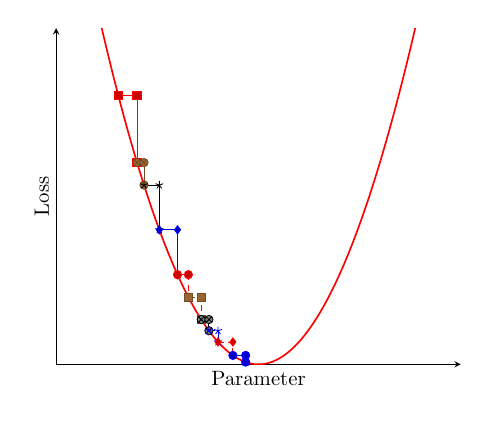
\begin{tikzpicture}[scale=0.75]
\begin{axis}[
        axis lines = left,
        xmin = 0,
        xmax = 10,
        xlabel = Parameter,
        ylabel = Loss,
        ticks = none
    ]
    \addplot [
        domain=1.12702:8.87298,
        samples=100,
        color=Red,
        thick
    ] {x^2 - 10*x + 25};
    \addplot coordinates {(1.5359,12) (2,12) (2,9)};
    \addplot coordinates {(2,9) (2.17157,9) (2.17157,8)};
    \addplot coordinates {(2.17157,8) (2.55051,8) (2.55051,6)};
    \addplot coordinates {(2.55051,6) (3,6) (3,4)};
    \addplot coordinates {(3,4) (3.26795,4) (3.26795,3)};
    \addplot coordinates {(3.26795,3) (3.58579,3) (3.58579,2)};
    \addplot coordinates {(3.58579,2) (3.77526,2) (3.77526,1.5)};
    \addplot coordinates {(3.77526,1.5) (4,1.5) (4,1)};
    \addplot coordinates {(4,1) (4.36754,1) (4.36754,0.4)};
    \addplot coordinates {(4.36754,0.4) (4.68377,0.4) (4.68377,0.1)};
\end{axis}
\end{tikzpicture}
\caption{Visualization of Case II}
\label{Visualization of Case II}
\end{figure}
\end{minipage}

Taking a look at Figure \ref{Visualization of Case I}, imagine your
random point in the red square. Because the slope of the line
tangent to the point in negative, you want to move to the right,
or in positive direction. This time, your learning rate is high that
the slope of the line tangent to the next landing position is
positive. Therefore, you want to move to the left, which is the
negative direction. After continuing this process over and over again
while adjusting the learning rate, you will likely find the local
minimum. In Figure \ref{Visualization of Case II}, our learning
rate is low. Despite being low, it will still lead to the local
minimum. One thing to note is that you don't want your learning rate
to be low or high as you might need to train forever or overshoot.
Learning rate is often denoted as $\eta$, and we normally would
adjust it with the gradient, which we will see in a bit. Of course
in real training, we won't be finding the slope of the tangent line as
we do in the 2-dimensional plane. In higher dimension, we would find
the gradient. Please refer to the first note for more information!

Another very popular analogy is foggy mountain analogy. Imagine you
are in the top of the mountain, and its getting dark. You want to
get to the lowest point as fast as possible. However, you can't see
anything beyond your local information because the mountain is very
foggy. What would you do? We would find the gradient and multiply
it with the learning rate to determine our step size. Then, with
your local information, we would be able to approach the local
minimum of the foggy mountain. Ideally, we should be hoping that
we reach the lowest point and villages.

Now, before we continue for building our own neural net without
machine learning libraries, let's conclude the concepts by
discussing different types of gradient descent and their effects.

\subsubsection{Types of Gradient Descent}

There are many types of gradient descents like Batch GD,
Mini-batch GD, Stochastic GD, and Momentum-Based GD. However,
the three major types are Batch Gradient Descent (BGD), Stochastic
Gradient Descent (SGD), and Mini-batch Gradient Descent. On the
high level, consider the following definitions.

\begin{definition}{}{}
With \textbf{Batch Gradient Descent (BGD)}, each update will
occur based on the entire training examples, which are often
averaged. In contrast, \textbf{Stochastic Gradient Descent (SGD)}
updates based on a single data point. \textbf{Mini-batch Gradient
Descent} is the middle ground of BGD and SGD that it updates based
on few data points like $32$ or $64$, usually in a power of $2$.
\end{definition}

From the sense, we can notice that the biggest difference in use case
would be efficiency and accuracy. BGD is generally more accurate in
each update than SGD as it is based on the entire data points.
However, SGD is generally more efficient as it does not have to
perform massive computations for each update to incorporate all the
training examples. One interesting thing to note is that because
SGD is ``stochastic'', or more noisy, it is sometimes better at
optimizing the updates as it moves more randomly than BGD.

When visualizing, we often consider the following diagram.

\begin{figure}[H]
\centering
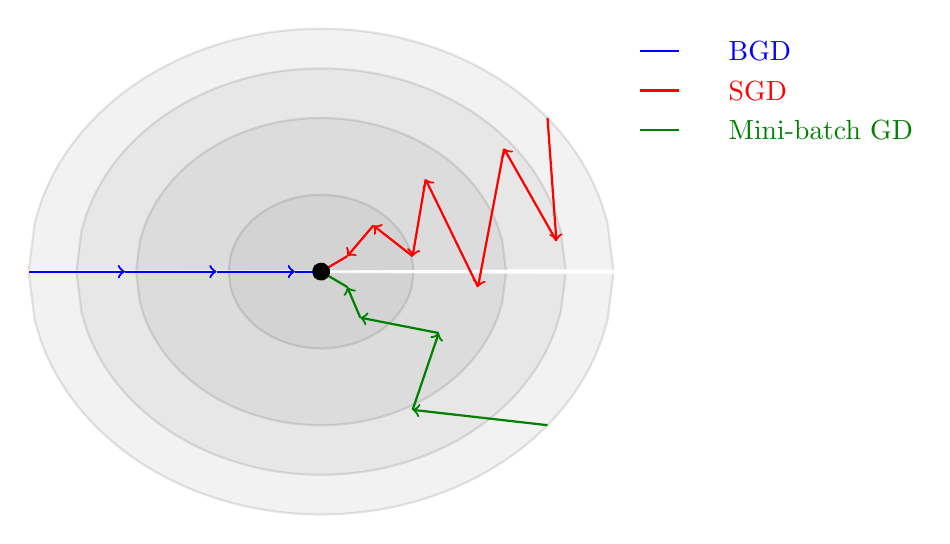
\begin{tikzpicture}
    \begin{axis}[
            axis lines = none,
            ticks=none,
            scale=1.3,
            bgd/.style={->,thick,Blue},
            sgd/.style={->,thick,Red},
            mini/.style={->,thick,Green},
        ]

        \addplot[thick, domain=-sqrt(5):sqrt(5),
                 samples=100, fill=Gray, opacity=0.1]
            {sqrt((5-x^2)/2)};
        \addplot[thick, domain=-sqrt(5):sqrt(5),
                 samples=100, fill=Gray, opacity=0.1]
            {-sqrt((5-x^2)/2)};

        \addplot[thick, domain=-sqrt(3.5):sqrt(3.5),
                 samples=100, fill=Gray, opacity=0.1]
            {sqrt((3.5-x^2)/2)};
        \addplot[thick, domain=-sqrt(3.5):sqrt(3.5),
                 samples=100, fill=Gray, opacity=0.1]
            {-sqrt((3.5-x^2)/2)};

        \addplot[thick, domain=-sqrt(2):sqrt(2),
                 samples=100, fill=Gray, opacity=0.1]
            {sqrt((2-x^2)/2)};
        \addplot[thick, domain=-sqrt(2):sqrt(2),
                 samples=100, fill=Gray, opacity=0.1]
            {-sqrt((2-x^2)/2)};

        \addplot[thick, domain=-sqrt(0.5):sqrt(0.5),
                 samples=100, fill=Gray, opacity=0.1]
            {sqrt((0.5-x^2)/2)};
        \addplot[thick, domain=-sqrt(0.5):sqrt(0.5),
                 samples=100, fill=Gray, opacity=0.1]
            {-sqrt((0.5-x^2)/2)};

        \addplot[mark=*, mark size=3pt] coordinates {(0,0)};

        \addplot[bgd] coordinates {(-sqrt(5),0) (-1.5,0)};
        \addplot[bgd] coordinates {(-1.5,0) (-0.8,0)};
        \addplot[bgd] coordinates {(-0.8,0) (-0.2,0)};
        \addplot[bgd] coordinates {(-0.2,0) (0,0)};

        \addplot[sgd] coordinates {(sqrt(3),1) (1.8,0.2)};
        \addplot[sgd] coordinates {(1.8,0.2) (1.4,0.8)};
        \addplot[sgd] coordinates {(1.4,0.8) (1.2,-0.1)};
        \addplot[sgd] coordinates {(1.2,-0.1) (0.8,0.6)};
        \addplot[sgd] coordinates {(0.8,0.6) (0.7,0.1)};
        \addplot[sgd] coordinates {(0.7,0.1) (0.4,0.3)};
        \addplot[sgd] coordinates {(0.4,0.3) (0.2,0.1)};
        \addplot[sgd] coordinates {(0.2,0.1) (0,0)};

        \addplot[mini] coordinates {(sqrt(3),-1) (0.7,-0.9)};
        \addplot[mini] coordinates {(0.7,-0.9) (0.9,-0.4)};
        \addplot[mini] coordinates {(0.9,-0.4) (0.3,-0.3)};
        \addplot[mini] coordinates {(0.3,-0.3) (0.2,-0.1)};
        \addplot[mini] coordinates {(0.2,-0.1) (0,0)};
    \end{axis}
    \begin{scope}[shift={(8.5,5.5)}]
        \draw[-,thick,Blue] (0,1) -- (0.5,1)
            node[right] at (1,1) {BGD};
        \draw[-,thick,Red] (0,0.5) -- (0.5,0.5)
            node[right] at (1,0.5) {SGD};
        \draw[-,thick,Green] (0,0) -- (0.5,0)
            node[right] at (1,0) {Mini-batch GD};
    \end{scope}
\end{tikzpicture}
\caption{Visualization of Different Types of Gradient Descent}
\end{figure}

As you can see, BGD often heads straightly towards the minimum
as the entire training examples are incorporated. Unlike BGD,
SGD shows more random and noisy movement and often requires more
updates to reach the local minimum. Finally, Mini-batch GD is
like the movement in between those two. Its is some what random,
but less noisy SGD that it often requires less updates.

Overall, this is what artificial neural nets are about.
The pre-trained and inter-connected neurons work together to
predict that output as a giant function. This giant function are
composed of weights and biases, which are fine-tuned during the
training process. During training, you calculate the loss and
tweak the parameters to minimize the loss through gradient descent.
You repeat the training process until your model learned well enough,
but not too much to prevent overfitting. That's pretty much it in
the high level! For our next section, let's discuss more on training
and gradient descent before we actually try and build a neural
network from scratch without ML libraries like PyTorch and TensorFlow.

Congratulations! We just finished the high level overview of what
neural nets are and what vanilla neural nets are composed of.
Before we actually try and implement the concepts with Python to
build a vanilla neural net without machine learing libraries like
PyTorch and TensorFlow, let's take a look at mathematical equations
to write them in code.

\end{document}


